\documentclass[11pt]{amsart}

\usepackage[T1]{fontenc}
\usepackage{lmodern}
\usepackage{amssymb,amsmath}
\usepackage{graphicx}
\usepackage{booktabs}
\usepackage{array}
\usepackage{xcolor}
\usepackage[margin=1.15in]{geometry}
\usepackage[colorlinks=true,linkcolor=blue!50!black,citecolor=blue!50!black,urlcolor=blue!50!black]{hyperref}

\newtheorem{theorem}{Theorem}[section]
\newtheorem{proposition}[theorem]{Proposition}
\newtheorem{lemma}[theorem]{Lemma}
\newtheorem{corollary}[theorem]{Corollary}
\newtheorem{thmx}{Theorem}
\renewcommand{\thethmx}{\Alph{thmx}}
\theoremstyle{definition}
\newtheorem{definition}[theorem]{Definition}
\newtheorem{example}[theorem]{Example}
\newtheorem{question}[theorem]{Question}
\theoremstyle{remark}
\newtheorem{remark}[theorem]{Remark}

\numberwithin{equation}{section}

\newcommand{\doi}[1]{\href{https://doi.org/#1}{\nolinkurl{doi:#1}}}
\newcommand{\Q}{\mathbb{Q}}
\newcommand{\Z}{\mathbb{Z}}
\newcommand{\F}{\mathbb{F}}
\newcommand{\cA}{\mathcal{A}}
\newcommand{\cO}{\mathcal{O}}
\newcommand{\Cay}{\operatorname{Cay}}
\newcommand{\Res}{\operatorname{Res}}
\newcommand{\disc}{\operatorname{disc}}
\newcommand{\rad}{\operatorname{J}}
\newcommand{\bK}{\overline{K}}
\hypersetup{pdftitle={Modular and integral spectral algebras of abelian Cayley graphs},pdfauthor={Deep Bhattacharjee}}

\begin{document}

\title[Modular and integral spectral algebras]{Modular and integral spectral algebras\\ of abelian Cayley graphs}

\author{Deep Bhattacharjee}
\address{Formerly, Electro-Gravitational Space Propulsion Laboratory (EGSPL),\newline Bhubaneswar, Odisha 751030, India}
\email{d.bhattacharjee@erl-forschung.de}
\email{itsdeep@live.com}
\urladdr{https://orcid.org/0000-0003-0466-750X}
\thanks{Corresponding author: \href{mailto:d.bhattacharjee@erl-forschung.de}{d.bhattacharjee@erl-forschung.de}; ORCID \href{https://orcid.org/0000-0003-0466-750X}{\mbox{0000-0003-0466-750X}}}

\subjclass[2020]{Primary 05C50; Secondary 05C25, 11R18, 16S34}
\keywords{Cayley graph, adjacency algebra, group algebra, Jacobson radical, real cyclotomic field, resultant, order, index}

\begin{abstract}
The algebra generated by the adjacency matrix of a Cayley graph on a finite abelian group is semisimple in characteristic $p$ exactly when every element of the connection set has order prime to $p$. For cycles we find its minimal polynomial in every characteristic and the index of the integral algebra in the maximal order, and we show that a prism over an $m$-cycle has as many distinct eigenvalues as an abelian group of order $2m$ allows if and only if neither $4$ nor $6$ divides $m$.
\end{abstract}

\maketitle

\section{Introduction}

Let $G$ be a finite abelian group of order $N$, let $S\subseteq G\setminus\{0\}$, and let $\Gamma=\Cay(G,S)$ be the Cayley graph with an arc from $g$ to $g+s$ for every $g\in G$ and $s\in S$. For a commutative ring $R$, the \emph{spectral algebra} $\cA_R(\Gamma)=R[A]$ is the subalgebra of $G\times G$ matrices over $R$ generated by the adjacency matrix $A$ of $\Gamma$. When $S=-S$ and $K$ is a field whose characteristic does not divide $N$, the structure of $\cA_K(\Gamma)$ is given by the character-orbit decomposition of Bhattacharjee, Mandal and Bhattacharya~\cite[Theorem~6.1]{BMB}: it is a product of fields, one for each orbit of $\operatorname{Gal}(\bK/K)$ on the eigenvalues
\[
\lambda_\chi=\sum_{s\in S}\chi(s),\qquad \chi\in\widehat G .
\]
Two cases lie outside that theorem: fields whose characteristic divides $N$, and the integral algebra $\cA_\Z(\Gamma)=\Z[A]$, which is an order in $\cA_\Q(\Gamma)$. This paper treats both, and answers two questions about the rational algebra raised in~\cite{BMB}.

\subsection*{Characteristic \texorpdfstring{$p$}{p}} Write $G=G_{p'}\times G_p$, where $G_p$ is the Sylow $p$-subgroup and $G_{p'}$ consists of the elements of order prime to $p$, and let $\pi\colon G\to G_{p'}$ be the projection. The \emph{shadow} of $\Gamma$ is the Cayley multigraph $\Gamma_{p'}=\Cay(G_{p'},\pi(S))$, in which $h$ is joined to $h+\pi(s)$ once for every $s\in S$.

\begin{thmx}\label{thm:A}
Let $K$ be a field of characteristic $p>0$ and let $q$ be a power of $p$ that is divisible by the exponent of $G_p$ and congruent to $1$ modulo the exponent of $G_{p'}$. Then $A^q=\sum_{s\in S}T_{\pi(s)}$ is the adjacency matrix of $\Cay(G,\pi(S))$, a disjoint union of $|G_p|$ copies of the shadow $\Gamma_{p'}$, the matrix $A-A^q$ is nilpotent, and
\[
\rad\bigl(\cA_K(\Gamma)\bigr)=(A-A^q)\,\cA_K(\Gamma),\qquad \cA_K(\Gamma)/\rad\bigl(\cA_K(\Gamma)\bigr)\cong \cA_K(\Gamma_{p'}).
\]
In particular $\cA_K(\Gamma)$ is semisimple if and only if every element of $S$ has order prime to $p$.
\end{thmx}

Here $\rad$ is the Jacobson radical. The description of the quotient is~\cite[Proposition~14.4]{BMB}; the new points are that the radical is principal with an explicit generator and the semisimplicity criterion, which needs neither $S=-S$ nor $S$ to generate $G$. A connected Cayley graph is semisimple in characteristic $p$ exactly when $p\nmid N$, but a disconnected one can be semisimple when $p\mid N$: the perfect matching $\Cay(\Z/6,\{3\})$ is semisimple over $\F_3$.

For cycles $C_n=\Cay(\Z/n,\{\pm1\})$ the radical can be described completely. Let $\Psi_d\in\Z[x]$ be the minimal polynomial of $2\cos(2\pi/d)$, so that $\Psi_1=x-2$, $\Psi_2=x+2$ and $\deg\Psi_d=\varphi(d)/2$ for $d\ge3$. Over $\Q$ the minimal polynomial of $A_{C_n}$ is $\prod_{d\mid n}\Psi_d$ (Lehmer~\cite{Le}, Watkins and Zeitlin~\cite{WZ}).

\begin{thmx}\label{thm:B}
Let $n=p^a m\ge3$ with $a\ge1$ and $p\nmid m$, put $q=p^a$, and let $K$ have characteristic $p$. The minimal polynomial of $A_{C_n}$ over $K$ is
\[
\prod_{d\mid m}\overline{\Psi}_d(x)^{e_d},\qquad e_d=\begin{cases} q, & d\ge3,\\ \lceil q/2\rceil, & d\le2,\end{cases}
\]
where $\overline{\Psi}_d$ is the reduction of $\Psi_d$ modulo $p$; these reductions are separable and pairwise coprime. Hence $\dim_K\cA_K(C_n)=\lfloor n/2\rfloor+1$ if $p$ is odd and $\dim_K\cA_K(C_n)=n/2$ if $p=2$.
\end{thmx}

So for odd $p$ the minimal polynomial over $\F_p$ is the reduction of the rational one, while for $p=2$ the reduction carries one superfluous factor $x$. Section~\ref{sec:integral} explains this through the integral algebra.

\subsection*{The integral algebra of a cycle} The rational algebra $\cA_\Q(C_n)\cong\prod_{d\mid n}\Q(\zeta_d)^+$ has the maximal order $\cO_n=\prod_{d\mid n}\cO_{\Q(\zeta_d)^+}$, and $\Z[A_{C_n}]$ is a suborder of finite index
\[
I(n)=\bigl[\cO_n:\Z[A_{C_n}]\bigr].
\]
The last display of~\cite{BMB} records the inclusion and leaves the index open.\footnote{It states that $\Z[A_{C_n}]=\cO_n$ ``in many (but not all) cases''. Theorem~\ref{thm:C}(ii) shows that equality never holds for $n\ge3$. The examples $n=3,4,5$ give $I(n)=3,16,5$.} For $d\ge1$ put $\varepsilon_d=1$ if $d\le2$ and $\varepsilon_d=2$ if $d\ge3$, and write $n_{p'}$ for the largest divisor of $n$ prime to $p$.

\begin{thmx}\label{thm:C}
Let $n\ge3$.
\begin{enumerate}
\item[(i)] $I(n)=\prod p^{\,2\varphi(d)/(\varepsilon_d\varepsilon_{d'})}$, the product taken over all pairs $d\mid d'\mid n$ with $d'/d$ a power $p^k$, $k\ge1$, of a prime $p$.
\item[(ii)] For a prime $p$ with $p^a\,\|\,n$, $a\ge1$,
\[
v_p\bigl(I(n)\bigr)=\begin{cases}\dfrac{n-n_{p'}}{2(p-1)}+\dfrac{a\gcd(2,n)}{2}, & p \text{ odd},\\[2ex] \dfrac{n-n_{2'}+2a+1}{2}, & p=2,\end{cases}
\]
and $p\nmid I(n)$ when $p\nmid n$. In particular $\Z[A_{C_n}]$ is never the maximal order.
\item[(iii)] $\Z[A_{C_n}]$ has index $\gcd(2,n)$ in the ring of symmetric integer circulant matrices, which is $\cA_\Q(C_n)\cap M_n(\Z)$.
\end{enumerate}
\end{thmx}

For instance $I(30)=2^9\cdot3^6\cdot5^4$, read off the edges of the divisor cube of $30$ in Figure~\ref{fig:cube}. The proof combines a resultant identity for the polynomials $\Psi_d$, which for $d,d'\ge3$ is due to Loper and Werner~\cite{LW}, with Apostol's evaluation of resultants of cyclotomic polynomials~\cite{Ap}.

\subsection*{The dimension of the rational algebra} Since $\lambda_\chi=\lambda_{\bar\chi}$, the dimension of $\cA_\Q(\Gamma)$, which is the number of distinct eigenvalues, is at most the number of orbits of $\chi\mapsto\bar\chi$ on $\widehat G$:
\begin{equation}\label{eq:bound}
\dim_\Q\cA_\Q(\Gamma)\le\frac{N+t}{2},\qquad t=\#\{g\in G:2g=0\}.
\end{equation}
This is~\cite[Remark~21.4]{BMB}, which leaves open whether noncyclic groups attain it; cycles do~\cite[Theorem~21.3]{BMB}. On the other hand \cite[Remark~19.4]{BMB} asserts the cyclic value $\lfloor N/2\rfloor+1$ as an upper bound for every group. The prism $C_m\,\square\,K_2=\Cay(\Z/m\times\Z/2,\{(\pm1,0),(0,1)\})$ settles both points.

\begin{thmx}\label{thm:D}
The prism $C_m\,\square\,K_2$, $m\ge3$, attains~\eqref{eq:bound} if and only if $4\nmid m$ and $6\nmid m$.
\end{thmx}

For $m\equiv2\pmod4$ with $3\nmid m$ the group $\Z/m\times\Z/2$ is not cyclic, the bound is attained, and the dimension $m+2$ exceeds $\lfloor 2m/2\rfloor+1=m+1$. The smallest case is the decagonal prism with $12$ distinct eigenvalues (Figure~\ref{fig:prism}). In the other direction, elementary abelian $2$- and $3$-groups of rank at least two never attain~\eqref{eq:bound} (Proposition~\ref{prop:elem}).

Section~\ref{sec:prelim} fixes notation. Sections~\ref{sec:modular}, \ref{sec:integral} and~\ref{sec:dimension} prove Theorems~\ref{thm:A} and~\ref{thm:B}, Theorem~\ref{thm:C}, and Theorem~\ref{thm:D}. Section~\ref{sec:type} records two facts about isomorphism types that correct statements in~\cite{BMB}.

Related work: Mönius determined the algebraic degree~\cite{Mo1} and the splitting field~\cite{Mo2} of the spectrum of a circulant graph, and Babai~\cite{Ba} described the spectra of Cayley graphs through characters. We use~\cite{BH} for background on graph spectra and~\cite{Wa} for cyclotomic fields.

\section{Preliminaries}\label{sec:prelim}

\subsection{The group algebra} For a commutative ring $R$ let $R[G]$ be the group algebra with basis $\{e_g:g\in G\}$ and $e_ge_h=e_{g+h}$. The regular representation $e_g\mapsto T_g$, where $T_g$ is the permutation matrix of $x\mapsto x+g$, is an injective algebra homomorphism $R[G]\to M_G(R)$, and $A=\sum_{s\in S}T_s$. Hence $\cA_R(\Gamma)\cong R[a]$ with
\[
a=\sum_{s\in S}e_s\in R[G],
\]
and the minimal polynomial of $A$ over a field is that of $a$ in the group algebra. For a multiset $S$ the same formula defines the adjacency matrix of the Cayley multigraph; this is how the shadow in Theorem~\ref{thm:A} is to be read.

\subsection{Cyclotomic notation} For $d\ge1$ let $\zeta_d=e^{2\pi i/d}$, let $\Phi_d$ be the $d$-th cyclotomic polynomial, and let $\Psi_d$ be the minimal polynomial of $\zeta_d+\zeta_d^{-1}=2\cos(2\pi/d)$ over $\Q$. Then $\Psi_d$ is monic with integer coefficients~\cite{Le}, of degree $\varphi(d)/\varepsilon_d$, and
\begin{equation}\label{eq:Psi-roots}
\Psi_d(x)^{\varepsilon_d}=\prod_{\substack{1\le j\le d\\ \gcd(j,d)=1}}\bigl(x-\zeta_d^{\,j}-\zeta_d^{-j}\bigr),
\end{equation}
since $j$ and $d-j$ give the same root and are distinct exactly when $d\ge3$. The ring of integers of $\Q(\zeta_d)^+=\Q(\zeta_d+\zeta_d^{-1})$ is $\Z[\zeta_d+\zeta_d^{-1}]\cong\Z[x]/(\Psi_d)$; see~\cite[Proposition~2.16]{Wa} and~\cite{Li}. The eigenvalues of $C_n$ are $2\cos(2\pi k/n)$, $0\le k<n$, so
\begin{equation}\label{eq:mCn}
m_{C_n}(x)=\prod_{d\mid n}\Psi_d(x),\qquad \cA_\Q(C_n)\cong\prod_{d\mid n}\Q(\zeta_d)^+,\qquad \dim_\Q\cA_\Q(C_n)=\lfloor n/2\rfloor+1 .
\end{equation}

\section{Characteristic \texorpdfstring{$p$}{p}}\label{sec:modular}

Throughout this section $K$ has characteristic $p>0$, $H=G_{p'}$, $P=G_p$, and $q$ is as in Theorem~\ref{thm:A}. Such $q$ exist: if $p^b$ is the exponent of $P$ and $r$ is the order of $p$ modulo the exponent of $H$, any $p^k$ with $r\mid k$ and $k\ge b$ will do.

\begin{proof}[Proof of Theorem~\ref{thm:A}]
Every element of $G$ is $g=\pi(g)+\rho(g)$ with $\rho(g)\in P$, and $qg=\pi(g)$ because $q\rho(g)=0$ and $q\pi(g)=\pi(g)$. Since $K[G]$ is commutative of characteristic $p$, the $q$-th power map is additive, and the coefficients of $a$ lie in the prime field, so
\[
a^q=\sum_{s\in S}e_{qs}=\sum_{s\in S}e_{\pi(s)}=:a_s .
\]
This element of $K[H]\subseteq K[G]$ is the one attached to the shadow, and it lies in $K[a]$.

Put $a_n=a-a_s=\sum_{s\in S}e_{\pi(s)}\bigl(e_{\rho(s)}-1\bigr)$. The augmentation ideal of $K[P]$ is generated by the elements $e_x-1$, $x\in P$, which satisfy $(e_x-1)^{p^b}=e_{p^bx}-1=0$. Since $K[G]$ is commutative, the ideal of $K[G]$ generated by these elements is nilpotent, and $a_n$ lies in it. Expanding polynomials in $a=a_s+a_n$ gives
\[
K[a]=K[a_s]+a_n K[a].
\]
The ideal $a_nK[a]$ is nilpotent, hence contained in $\rad(K[a])$. On the other hand $K[a_s]$ is a subalgebra of $K[H]$, which is a product of fields after extending scalars because $p\nmid|H|$ (Maschke's theorem); so $K[a_s]$ has no nonzero nilpotent elements. Its intersection with $a_nK[a]$ consists of nilpotent elements and is therefore zero, so $K[a]/a_nK[a]\cong K[a_s]$. A finite-dimensional commutative algebra without nilpotents is semisimple, which gives $\rad(K[a])=a_nK[a]$ and the description of the quotient.

Finally $K[a]$ is semisimple if and only if $a_n=0$, that is, $\sum_{s\in S}e_s=\sum_{s\in S}e_{\pi(s)}$. The right side is supported on $H$. If some $s_0\in S$ lies outside $H$, the coefficient of $e_{s_0}$ is $1$ on the left and $0$ on the right. If $S\subseteq H$, then $\pi(s)=s$ for every $s$ and the two sides agree.
\end{proof}

\begin{remark}\label{rem:jordan}
In matrix language $A=A^q+(A-A^q)$ is the Jordan--Chevalley decomposition of $A$, with both parts polynomials in $A$ over the prime field. The proof also gives $\dim_K\rad(\cA_K(\Gamma))=\deg m_{\Gamma,K}-\deg m_{\Gamma_{p'},K}$, where $m_{\Gamma,K}$ is the minimal polynomial over $K$. When $S$ generates $G$, the set $S\subseteq H$ forces $H=G$, so a connected Cayley graph is semisimple in characteristic $p$ exactly when $p\nmid N$; for cycles this is also observed in~\cite{BMBc}.
\end{remark}

\begin{example}\label{ex:charp}
Over $\F_3$, the graph $\Cay(\Z/6,\{3\})$ has $A^2=I$ and minimal polynomial $(x-1)(x+1)$, which is separable: $3$ has order $2$. The graph $\Cay(\Z/6,\{2,4\})$, two disjoint triangles, has $A^2=A+2I$, so $m(x)=x^2-x-2=(x+1)^2$ over $\F_3$, and $q=3$ gives $A^3=2I$, the adjacency matrix of the shadow $\Cay(\Z/2,\{0,0\})$, which has two loops at each vertex, with $\rad=(A-A^3)\F_3[A]=(A+I)\F_3[A]$.
\end{example}

\begin{proof}[Proof of Theorem~\ref{thm:B}]
The minimal polynomial does not change under field extension, so we may assume $K$ algebraically closed. Write $\Z/n=H\times P$ with $H\cong\Z/m$ and $P\cong\Z/q$, and let $g=(h_0,x_0)$ be the image of $1$. Put $y=e_{x_0}-1$; then $K[P]=K[y]/(y^q)$, because $y^q=e_{qx_0}-1=0$ and $K[P]$ has dimension $q$. The characters $\psi$ of $H$ with values in $K$ correspond bijectively to $\zeta=\psi(h_0)$ in the group $\mu_m(K)$ of $m$-th roots of unity, which has $m$ elements because $p\nmid m$, and
\[
K[G]=K[H]\otimes K[P]\;\xrightarrow{\ \sim\ }\;\prod_{\psi\in\widehat H}K[P],\qquad e_{h}\otimes u\mapsto\bigl(\psi(h)u\bigr)_\psi .
\]
The image of $a=e_g+e_{-g}$ in the factor of $\psi$ is $a_\psi=\zeta(1+y)+\zeta^{-1}(1+y)^{-1}$, and with $\lambda_\zeta=\zeta+\zeta^{-1}$ a short computation gives
\[
a_\psi-\lambda_\zeta=y(1+y)^{-1}\bigl((\zeta-\zeta^{-1})+\zeta y\bigr).
\]
If $\zeta^2\ne1$ the bracket is a unit, so $a_\psi-\lambda_\zeta$ is $y$ times a unit and has nilpotency index $q$. If $\zeta=\pm1$ then $a_\psi-\lambda_\zeta=\zeta y^2(1+y)^{-1}$ has nilpotency index $\lceil q/2\rceil$. The minimal polynomial of $a_\psi$ is therefore $(x-\lambda_\zeta)^{\nu_\zeta}$ with $\nu_\zeta\in\{q,\lceil q/2\rceil\}$ as just described, and the minimal polynomial of $a$ is the least common multiple of these over $\zeta\in\mu_m(K)$. Now $\lambda_\zeta=\lambda_\xi$ if and only if $\xi\in\{\zeta,\zeta^{-1}\}$, since $\zeta$ and $\zeta^{-1}$ are the roots of $x^2-\lambda_\zeta x+1$. So the minimal polynomial is $\prod(x-\lambda_\zeta)^{\nu_\zeta}$ over the pairs $\{\zeta,\zeta^{-1}\}$.

Group the pairs by the order $d\mid m$ of $\zeta$. In $\Z[\zeta_d][x]$ the polynomial $\Psi_d(x)$ is the product of $x-\omega-\omega^{-1}$ over the pairs $\{\omega,\omega^{-1}\}$ of primitive $d$-th roots of unity, and reduction modulo a prime above $p$ maps these roots bijectively onto the primitive $d$-th roots of unity in $K$, because $x^d-1$ is separable modulo $p$. So the product of $x-\lambda_\zeta$ over the pairs of order $d$ is $\overline{\Psi}_d$. Its roots are distinct, and different $d$ give coprime factors, because different pairs give different $\lambda_\zeta$. Since $\zeta^2=1$ exactly when $d\le2$, the exponents are $e_d$.

For the dimension let $t=\gcd(2,m)$ be the number of divisors $d\le2$ of $m$. The divisors $d\ge3$ contribute $\varphi(d)/2$ each, $(m-t)/2$ in all, so the degree of the minimal polynomial is
\[
t\lceil q/2\rceil+q(m-t)/2.
\] For odd $p$ this is $(n+t)/2=\lfloor n/2\rfloor+1$, because $t=\gcd(2,n)$. For $p=2$, $m$ is odd, $t=1$ and the degree is $q/2+q(m-1)/2=n/2$.
\end{proof}

\begin{corollary}\label{cor:reduction}
For odd $p$ the minimal polynomial of $A_{C_n}$ over $\F_p$ is $\prod_{d\mid n}\Psi_d$ reduced modulo $p$. For $p=2$ and even $n$ it is that reduction divided by $x$.
\end{corollary}

\begin{proof}
The reduction $\overline m$ of $m_{C_n}$ annihilates $A$, so the minimal polynomial over $\F_p$ divides it. For odd $p$ both are monic of degree $\lfloor n/2\rfloor+1$. For $p=2$ the quotient has degree one, so it suffices to compare the multiplicities of the root $0$. A root $\zeta+\zeta^{-1}$ of $\Psi_d$ reduces to $0$ modulo a prime above $2$ exactly when $\zeta$ reduces to $1$, that is, when $d$ is a power of $2$; so the multiplicity in $\overline m$ is $\sum_{b=0}^{a}\deg\Psi_{2^b}=2^{a-1}+1$, against $2^{a-1}$ in the minimal polynomial.
\end{proof}

\section{The integral algebra of a cycle}\label{sec:integral}

\subsection{Symmetric circulants} For $0\le k\le n/2$ let $c_k=T_k+T_{-k}$ if $0<k<n/2$, and $c_0=I$, $c_{n/2}=T_{n/2}$ when these are defined. The matrices $c_k$ have disjoint supports, and their $\Z$-span $\Z[C_n]^+$ is the ring of symmetric integer circulant matrices.

\begin{proposition}\label{prop:sym}
$\cA_\Q(C_n)$ is the $\Q$-span of $c_0,\dots,c_{\lfloor n/2\rfloor}$, so $\Z[C_n]^+=\cA_\Q(C_n)\cap M_n(\Z)$. If $n$ is odd then $\Z[A]=\Z[C_n]^+$. If $n$ is even then $\Z[A]$ is spanned by $c_0,\dots,c_{n/2-1}$ and $2c_{n/2}$, and has index $2$ in $\Z[C_n]^+$.
\end{proposition}

\begin{proof}
With $A=c_1$ we have
\[
Ac_k=c_{k+1}+c_{k-1}\quad(2\le k,\ k+1<n/2),\qquad Ac_1=c_2+2c_0\quad(2<n/2),
\]
and, for even $n$, $Ac_{n/2-1}=2c_{n/2}+c_{n/2-2}$ if $n\ge6$ and $Ac_1=2c_2+2c_0$ if $n=4$. By induction $A^j\in c_j+\Z c_0+\dots+\Z c_{j-1}$ for $j<n/2$, and $A^{n/2}\in 2c_{n/2}+\Z c_0+\dots+\Z c_{n/2-1}$ for even $n$. Because $m_{C_n}$ is monic of degree $\lfloor n/2\rfloor+1$, the powers $A^0,\dots,A^{\lfloor n/2\rfloor}$ form a $\Z$-basis of $\Z[A]$, and the triangular relations give both statements about $\Z[A]$. Tensoring with $\Q$ gives the first sentence.
\end{proof}

This explains Corollary~\ref{cor:reduction} from the integral side: the reduction map $\Z[A]\otimes\F_p\to M_n(\F_p)$ is injective exactly when $\Z[A]$ is saturated at $p$, which by Proposition~\ref{prop:sym} fails only for $p=2$ and even $n$, and then the kernel is spanned by the image of $2c_{n/2}$.

\subsection{Resultants} The next two lemmas are standard in substance; we include short proofs.

\begin{lemma}\label{lem:index}
Let $f_1,\dots,f_r\in\Z[x]$ be monic and pairwise coprime in $\Q[x]$, and $f=f_1\cdots f_r$. The natural map $\Z[x]/(f)\to\prod_i\Z[x]/(f_i)$ is injective with image of index $\prod_{i<j}|\Res(f_i,f_j)|$.
\end{lemma}

\begin{proof}
Take $r=2$, $f_1=u$, $f_2=v$. If $h\in\Z[x]$ is divisible by $u$ and by $v$ in $\Z[x]$, then $uv\mid h$ in $\Q[x]$, and division by the monic polynomial $uv$ shows that the quotient has integer coefficients; so the map is injective. The map $(\alpha,\beta)\mapsto\alpha-\beta$ from $\Z[x]/(u)\times\Z[x]/(v)$ onto $\Z[x]/(u,v)$ has kernel exactly the image, because $\alpha-\beta=u\gamma+v\delta$ means that $\alpha-u\gamma=\beta+v\delta$ is a common lift. Finally $\Z[x]/(u,v)=R/vR$ with $R=\Z[x]/(u)$ free of rank $\deg u$, and $|R/vR|$ is the absolute value of the determinant of multiplication by $v$ on $R$, which is $\prod_{u(\theta)=0}v(\theta)=\pm\Res(u,v)\ne0$. For $r>2$ factor the map through $\Z[x]/(f_1\cdots f_{r-1})\times\Z[x]/(f_r)$ and use $\Res(f_1\cdots f_{r-1},f_r)=\prod_{i<r}\Res(f_i,f_r)$.
\end{proof}

\begin{lemma}\label{lem:res}
For $d\ne d'$,
\[
|\Res(\Psi_d,\Psi_{d'})|^{\varepsilon_d\varepsilon_{d'}}=\Res(\Phi_d,\Phi_{d'})^2 .
\]
Consequently, for $d<d'$, $|\Res(\Psi_d,\Psi_{d'})|=p^{2\varphi(d)/(\varepsilon_d\varepsilon_{d'})}$ if $d'/d=p^k$ with $p$ prime and $k\ge1$, and $|\Res(\Psi_d,\Psi_{d'})|=1$ otherwise.
\end{lemma}

\begin{proof}
By~\eqref{eq:Psi-roots}, $\Res(\Psi_d,\Psi_{d'})^{\varepsilon_d\varepsilon_{d'}}$ is the product of $\alpha+\alpha^{-1}-\beta-\beta^{-1}$ over all primitive $d$-th roots $\alpha$ and primitive $d'$-th roots $\beta$. The identity
\[
\alpha+\alpha^{-1}-\beta-\beta^{-1}=(\alpha-\beta)\bigl(1-\alpha^{-1}\beta^{-1}\bigr)=-\beta^{-1}(\alpha-\beta)\bigl(\alpha^{-1}-\beta\bigr)
\]
and the fact that $\alpha\mapsto\alpha^{-1}$ permutes the primitive $d$-th roots show that this product is a root of unity times $\Res(\Phi_d,\Phi_{d'})^2$. Taking absolute values gives the identity. Apostol~\cite{Ap} proved that for $1\le d<d'$ the resultant $\Res(\Phi_d,\Phi_{d'})$ equals $p^{\varphi(d)}$ if $d'/d$ is a power of a prime $p$ and $1$ otherwise.\footnote{For $d=1$ this is the classical value $\Phi_{d'}(1)$.} The exponent $2\varphi(d)/(\varepsilon_d\varepsilon_{d'})$ is an integer because $\varphi(d)$ is even for $d\ge3$.
\end{proof}

For $d,d'\ge3$ the second statement is~\cite[Theorem~3.4]{LW}, where the sign of the resultant is also determined.

\subsection{Proof of Theorem~\ref{thm:C}}
By~\eqref{eq:mCn} and Section~\ref{sec:prelim} we have $\Z[A]\cong\Z[x]/(m_{C_n})$ and
\[
\cO_n\cong\prod_{d\mid n}\Z[x]/(\Psi_d),
\]
compatibly with the inclusion. Lemmas~\ref{lem:index} and~\ref{lem:res} give (i).

For (ii) fix $p$ with $p^a\,\|\,n$, $a\ge1$, write $m=n_{p'}$, and collect the pairs in (i) with $d'/d$ a power of $p$: they are $d=p^be$, $d'=p^ce$ with $e\mid m$ and $0\le b<c\le a$. If $e\ge3$ every $\varepsilon$ equals $2$ and the contribution is
\[
\frac{\varphi(e)}{2}\sum_{0\le b<c\le a}\varphi(p^b)=\frac{\varphi(e)}{2}\sum_{c=1}^{a}p^{c-1}=\frac{\varphi(e)}{2}\cdot\frac{p^a-1}{p-1}.
\]
Summing over $e\mid m$, $e\ge3$, gives $\frac{m-t}{2}\cdot\frac{p^a-1}{p-1}$ with $t=\gcd(2,m)$. If $e\le2$ and $p$ is odd, the pairs with $b=0$ contribute $1$ each, $a$ in all, and those with $b\ge1$ contribute $\varphi(p^b)/2$, in all $\frac12\sum_{c=1}^{a}(p^{c-1}-1)$; the total for one such $e$ is $\frac12\bigl(a+\frac{p^a-1}{p-1}\bigr)$. Adding up,
\[
v_p(I(n))=\frac{m-t}{2}\cdot\frac{p^a-1}{p-1}+\frac t2\Bigl(a+\frac{p^a-1}{p-1}\Bigr)=\frac{(p^a-1)\,m}{2(p-1)}+\frac{at}{2},
\]
which is the stated formula since $(p^a-1)m=n-n_{p'}$ and $t=\gcd(2,n)$ for odd $p$. For $p=2$ only $e=1$ has $e\le2$; its pairs contribute $2$ for $(b,c)=(0,1)$, $1$ for each $(0,c)$ and $(1,c)$ with $c\ge2$, and $2^{b-2}$ for each $(b,c)$ with $b\ge2$, in all $2+2(a-1)+\sum_{c=3}^{a}(2^{c-2}-1)=a+2^{a-1}$. Together with $(2^a-1)(m-1)/2$ from the odd $e\ge3$ this is $(n-m+2a+1)/2$. Both expressions are positive, so $I(n)>1$ whenever $n\ge3$; if $p\nmid n$ no pair in (i) involves $p$.

Part (iii) is Proposition~\ref{prop:sym}. \qed

\begin{corollary}
The discriminant of $m_{C_n}$ is $I(n)^2\prod_{d\mid n}\disc\bigl(\Q(\zeta_d)^+\bigr)$, the order $\Z[C_n]^+$ has index $I(n)/\gcd(2,n)$ in $\cO_n$, and
\[
\log I(n)=\frac n2\sum_{p\mid n}\Bigl(1-\frac{n_{p'}}{n}\Bigr)\frac{\log p}{p-1}+O(\log n).
\]
\end{corollary}

\begin{proof}
The first statement is the usual relation between discriminant and index~\cite[Chapter~I, (2.12)]{Ne}, applied factor by factor; the second follows from Theorem~\ref{thm:C}(iii); the third from (ii), since the terms $\frac{a}{2}\gcd(2,n)\log p$ and $\frac{2a+1}{2}\log 2$ add up to at most $\log n+1$.
\end{proof}

\begin{table}[ht]
\centering
\small
\renewcommand{\arraystretch}{1.15}
\begin{tabular}{>{$}r<{$}>{$}l<{$}@{\qquad}>{$}r<{$}>{$}l<{$}@{\qquad}>{$}r<{$}>{$}l<{$}}
\toprule
n & I(n) & n & I(n) & n & I(n)\\
\midrule
3 & 3 & 13 & 13 & 23 & 23\\
4 & 2^4 & 14 & 2^5\,7^2 & 24 & 2^{14}\,3^5\\
5 & 5 & 15 & 3^3\,5^2 & 25 & 5^4\\
6 & 2^3\,3^2 & 16 & 2^{12} & 26 & 2^8\,13^2\\
7 & 7 & 17 & 17 & 27 & 3^8\\
8 & 2^7 & 18 & 2^6\,3^6 & 28 & 2^{13}\,7^3\\
9 & 3^3 & 19 & 19 & 29 & 29\\
10 & 2^4\,5^2 & 20 & 2^{10}\,5^3 & 30 & 2^9\,3^6\,5^4\\
11 & 11 & 21 & 3^4\,7^2 & & \\
12 & 2^7\,3^3 & 22 & 2^7\,11^2 & & \\
\bottomrule
\end{tabular}
\caption{The index $I(n)=[\cO_n:\Z[A_{C_n}]]$ for $3\le n\le30$. Each value agrees with $\sqrt{|\disc(m_{C_n})|/\prod_{d\mid n}|\disc\Q(\zeta_d)^+|}$, computed independently for $n\le150$.}
\label{tab:index}
\end{table}

\begin{figure}[ht]
\centering
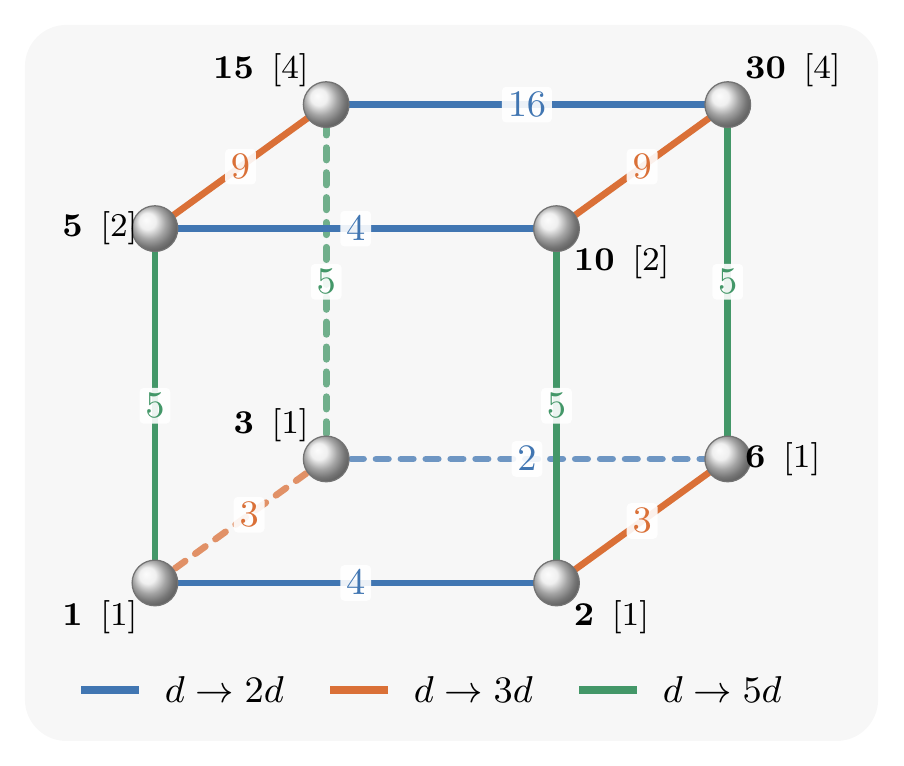
\includegraphics[width=0.62\textwidth]{figures/cube30.png}
\caption{The divisors of $30$ as a cube. The edge from $d$ to $pd$ carries $|\Res(\Psi_d,\Psi_{pd})|$, and the product of all twelve labels is $I(30)=2^9\cdot3^6\cdot5^4$. Vertices are labelled by $d$ and the degree of $\Q(\zeta_d)^+$.}
\label{fig:cube}
\end{figure}

\begin{figure}[ht]
\centering
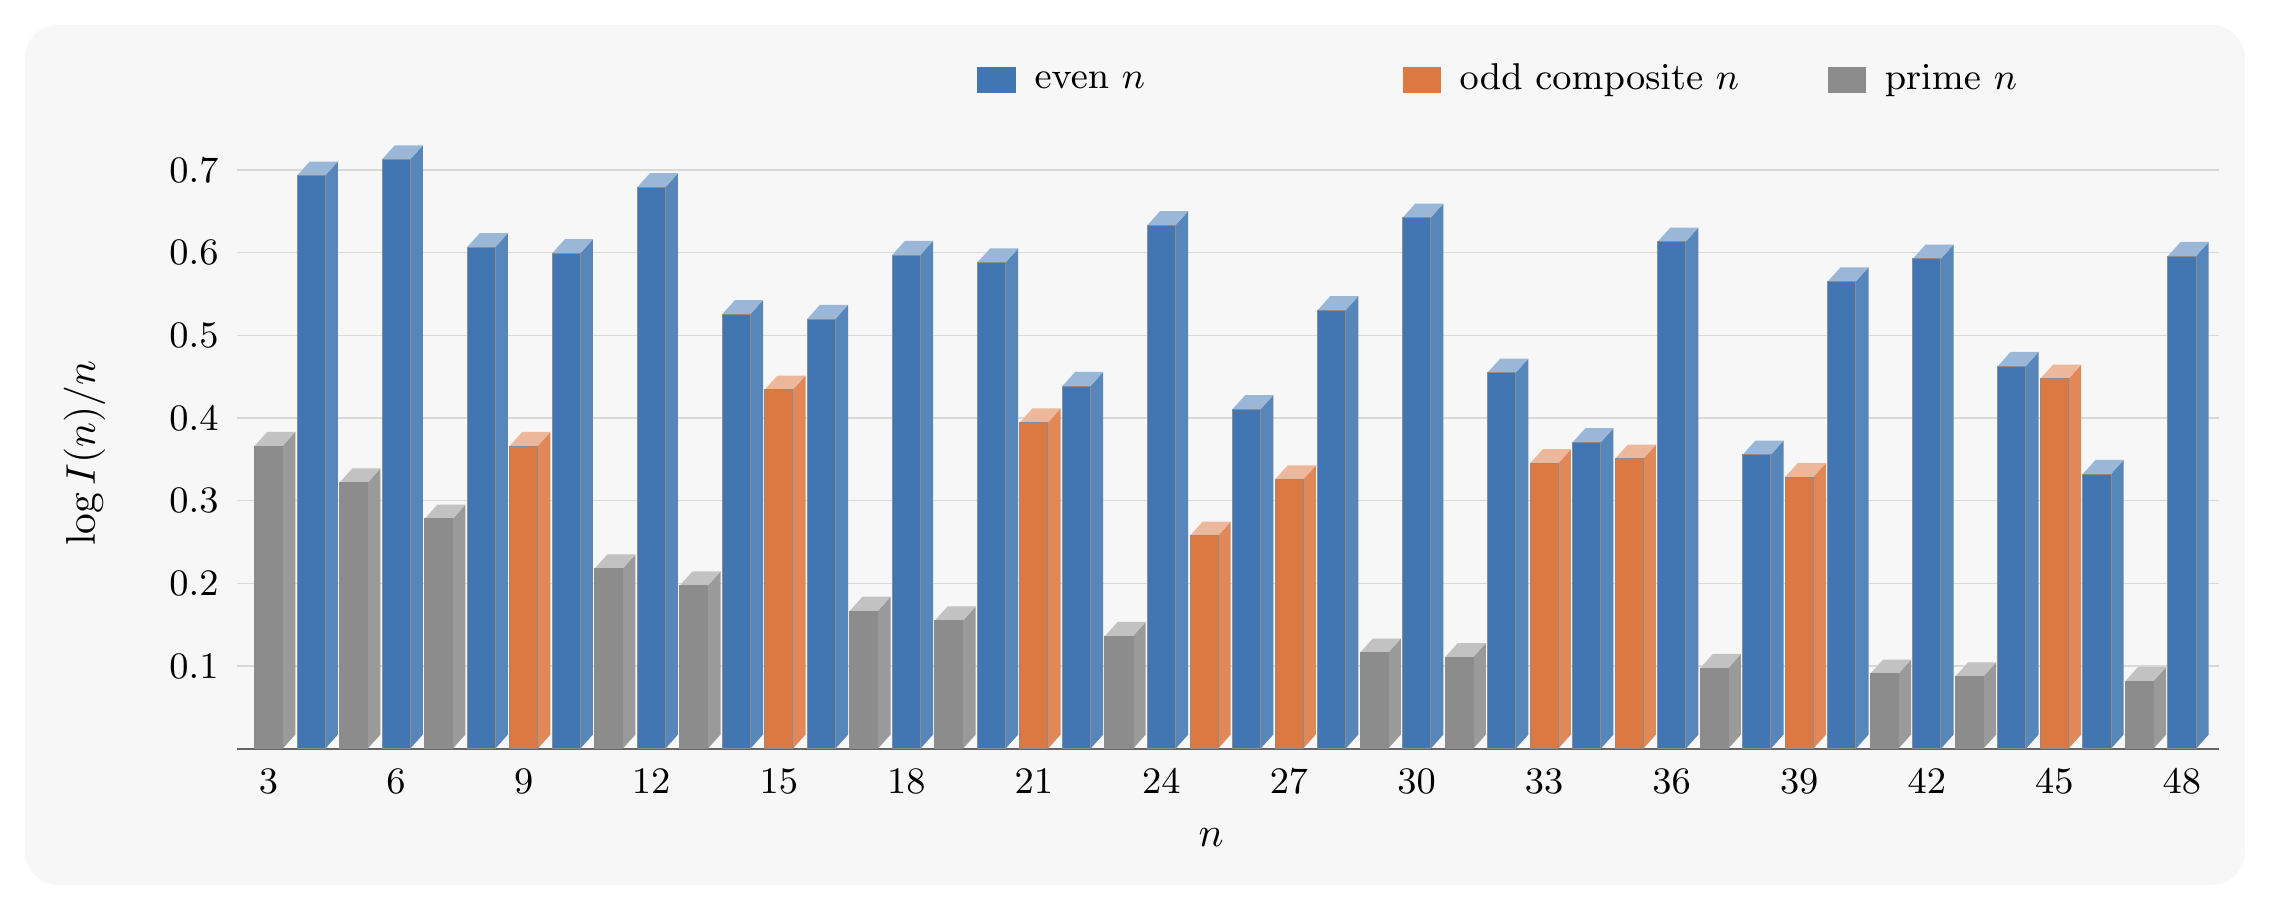
\includegraphics[width=0.86\textwidth]{figures/bars.png}
\caption{The normalized index $\log I(n)/n$ for $3\le n\le 48$. For prime $n$ the value is $(\log n)/n$; the largest values occur for even $n$ with several small prime factors.}
\label{fig:bars}
\end{figure}

\section{The dimension of the rational algebra}\label{sec:dimension}

Recall~\eqref{eq:bound}: $\widehat G\cong G$, and the characters fixed by $\chi\mapsto\bar\chi$ are those of order at most two, of which there are $t$; so the involution has $(N+t)/2$ orbits.

\begin{lemma}\label{lem:totpos}
Let $\gamma=2\cos(2\pi j/d)$ with $\gcd(j,d)=1$. Every Galois conjugate of $\gamma$ is $\ge0$ if and only if $d\in\{1,4,6\}$, and every conjugate is $\le0$ if and only if $d\in\{2,3,4\}$.
\end{lemma}

\begin{proof}
The conjugates are $2\cos(2\pi i/d)$ with $\gcd(i,d)=1$, and such a value is negative exactly when $d/4<i<3d/4$. For odd $d\ge3$ take $i=(d-1)/2$; for $d=2e$ with $e\ge4$ even take $i=e-1$, and with $e\ge5$ odd take $i=e-2$. In each case $\gcd(i,d)=1$ and $d/4<i<3d/4$, so some conjugate is negative. The remaining $d$ are $1,2,4,6$, with conjugates $\{2\}$, $\{-2\}$, $\{0\}$, $\{1\}$. For the second statement, $\cos(2\pi/d)\le0$ forces $d\le4$, and among $d=2,3,4$ the conjugates are $\{-2\}$, $\{-1\}$, $\{0\}$, while $d=1$ gives $2$.
\end{proof}

\begin{proof}[Proof of Theorem~\ref{thm:D}]
Here $N=2m$, and $t=4$ for even $m$ and $t=2$ for odd $m$, so $(N+t)/2=2(\lfloor m/2\rfloor+1)$. The eigenvalues of the prism are $\gamma_k\pm1$ with $\gamma_k=2\cos(2\pi k/m)$, $0\le k\le\lfloor m/2\rfloor$, and the $\gamma_k$ are distinct. So the bound is attained if and only if $\gamma_k+1\ne\gamma_j-1$ for all $j,k$, that is, no two of the $\gamma$'s differ by $2$. If $4\mid m$ then $\gamma_0-\gamma_{m/4}=2-0$, and if $6\mid m$ then $\gamma_{m/6}-\gamma_{m/3}=1-(-1)$. Conversely suppose $\gamma_j-\gamma_k=2$. For every automorphism $\sigma$ of $\Q(\zeta_m)$ we get $\sigma(\gamma_j)-\sigma(\gamma_k)=2$, and since every conjugate lies in $[-2,2]$ this forces $\sigma(\gamma_j)\ge0\ge\sigma(\gamma_k)$. By Lemma~\ref{lem:totpos}, $\gamma_j\in\{2,0,1\}$ and $\gamma_k\in\{-2,0,-1\}$, so $(\gamma_j,\gamma_k)$ is $(2,0)$, $(0,-2)$ or $(1,-1)$. The first two need an element of order $4$ in $\Z/m$, the third one of order $6$.
\end{proof}

\begin{figure}[ht]
\centering
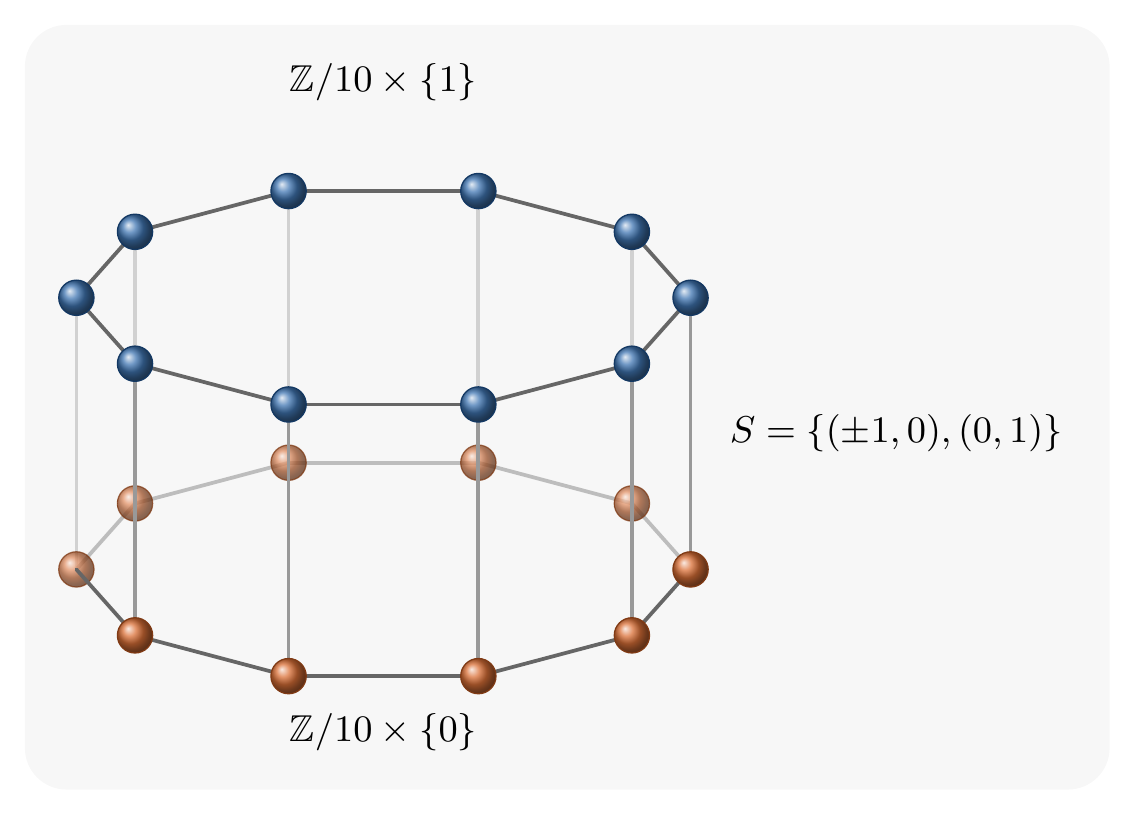
\includegraphics[width=0.62\textwidth]{figures/prism.png}
\caption{The decagonal prism $C_{10}\,\square\,K_2$ on $\Z/10\times\Z/2$. Its twelve distinct eigenvalues $\pm3$, $\pm1$, $\pm\phi$, $\pm(\phi+1)$, $\pm(\phi-1)$, $\pm(\phi-2)$, where $\phi=(1+\sqrt5)/2$, reach the bound $(20+4)/2$.}
\label{fig:prism}
\end{figure}

\begin{proposition}\label{prop:elem}
Let $k\ge2$. For $G=(\Z/2)^k$ every Cayley graph has $\dim_\Q\cA_\Q(\Gamma)\le2^{k-1}+1<2^k=(N+t)/2$. For $G=(\Z/3)^k$ every Cayley graph with $S=-S$ has $\dim_\Q\cA_\Q(\Gamma)\le(3^{k-1}+3)/2<(3^k+1)/2=(N+t)/2$. Both bounds are attained for $k=2$.
\end{proposition}

\begin{proof}
For $G=(\Z/2)^k$ and $\chi\ne1$, $\lambda_\chi=2|S\cap\ker\chi|-|S|$, and $|S\cap\ker\chi|$ lies between $0$ and $2^{k-1}-1$; with $\lambda_1=|S|$ there are at most $2^{k-1}+1$ values. For $G=(\Z/3)^k$ write $S=T\cup(-T)$ with $|T|=\ell$. Each $s\in T$ contributes $\chi(s)+\overline{\chi(s)}\in\{2,-1\}$, so $\lambda_\chi=3|T\cap\ker\chi|-\ell$, and for $\chi\ne1$ the count $|T\cap\ker\chi|$ is at most $(3^{k-1}-1)/2$, the number of pairs $\pm s$ in a hyperplane. With $\lambda_1$ this gives the bound. For $k=2$, $S=\{(1,0),(0,1)\}$ in $(\Z/2)^2$ has the eigenvalues $2,0,-2$, and $S=\{\pm(1,0),\pm(0,1)\}$ in $(\Z/3)^2$ has $4,1,-2$.
\end{proof}

Table~\ref{tab:maxdim} lists the largest dimension over all symmetric $S$ for small groups, found by exhaustive search. Apart from cyclic groups, only $\Z/2\times\Z/10$ reaches the bound in this range, in accordance with Theorem~\ref{thm:D}.

\begin{table}[ht]
\centering
\small
\renewcommand{\arraystretch}{1.15}
\begin{tabular}{lccc@{\qquad}lccc}
\toprule
$G$ & $N$ & max & $(N+t)/2$ & $G$ & $N$ & max & $(N+t)/2$\\
\midrule
$(\Z/2)^2$ & 4 & 3 & 4 & $\Z/2\times\Z/8$ & 16 & 9 & 10\\
$\Z/2\times\Z/4$ & 8 & 4 & 6 & $\Z/3\times\Z/6$ & 18 & 7 & 10\\
$(\Z/2)^3$ & 8 & 4 & 8 & $\Z/2\times\Z/10$ & 20 & 12 & 12\\
$(\Z/3)^2$ & 9 & 3 & 5 & $(\Z/2)^2\times\Z/4$ & 16 & 6 & 12\\
$\Z/2\times\Z/6$ & 12 & 7 & 8 & $(\Z/2)^4$ & 16 & 6 & 16\\
$\Z/4\times\Z/4$ & 16 & 6 & 10 & $\Z/2\times\Z/12$ & 24 & 13 & 14\\
$(\Z/5)^2$ & 25 & 10 & 13 & $\Z/3\times\Z/9$ & 27 & 13 & 14\\
\bottomrule
\end{tabular}
\caption{Largest number of distinct eigenvalues of $\Cay(G,S)$ over all symmetric $S\subseteq G\setminus\{0\}$, against the bound~\eqref{eq:bound}.}
\label{tab:maxdim}
\end{table}

\begin{question}
For which finite abelian groups is~\eqref{eq:bound} attained by some symmetric $S$?
\end{question}

\section{Isomorphism types}\label{sec:type}

Two finite products of number fields are isomorphic as $\Q$-algebras if and only if their factors agree up to isomorphism and multiplicity, because the factors are the localizations at the minimal primes. Hence $\cA_\Q(\Cay(G,S))\cong\cA_\Q(\Cay(G,S'))$ if and only if the multisets of fields $\Q(\lambda_O)$, $O$ running over the Galois orbits of eigenvalues, agree up to isomorphism. Equal orbit sizes are not enough.\footnote{This corrects the ``if'' direction of~\cite[Proposition~21.1]{BMB}.}

\begin{example}\label{ex:z24}
On $\Z/24$ take $S=\{\pm2\}$ and $S'=\{\pm1,\pm5\}$. The first graph is two copies of $C_{12}$, with algebra $\Q^5\times\Q(\sqrt3)$. For the second, $\lambda_k=2\cos(\pi k/12)+2\cos(5\pi k/12)=4\cos(\pi k/4)\cos(\pi k/6)$, which takes the rational values $4,0,2,-2,-4$ at $k=0,2,4,8,12$ and the values $\pm\sqrt6$ at $k=1,7$; the algebra is $\Q^5\times\Q(\sqrt6)$. Both have dimension $7$ and orbit sizes $1,1,1,1,1,2$, but they are not isomorphic.
\end{example}

\begin{proposition}\label{prop:type}
For $n\ge3$ the isomorphism type of the $\Q$-algebra $\cA_\Q(C_n)$ determines $n$.
\end{proposition}

\begin{proof}
The dimension $D=\lfloor n/2\rfloor+1$ leaves $n\in\{2D-2,2D-1\}$. Recall that $\Q(\zeta_d)^+=\Q$ for $d\le4$ and $d=6$, that $\Q(\zeta_d)^+=\Q(\zeta_{d/2})^+$ for $d\equiv2\pmod 4$, and that otherwise the conductor of $\Q(\zeta_d)^+$ is $d$.\footnote{The field $\Q(\zeta_d)^+$ is fixed by $\{\pm1\}\subseteq(\Z/d)^\times$, and it lies in $\Q(\zeta_f)$ for a proper divisor $f$ of $d$ only if the kernel of $(\Z/d)^\times\to(\Z/f)^\times$ is contained in $\{\pm1\}$. For $f\ge3$ this kernel does not contain $-1$, so it must be trivial, which forces $d=2f$ with $f$ odd; for $f\le2$ it is all of $(\Z/d)^\times$, which forces $\varphi(d)\le2$.} So every factor of $\cA_\Q(C_n)$ has conductor dividing $n$, and when $n$ is odd and $n\ge5$ the factor $\Q(\zeta_n)^+$ has conductor $n$. Thus $n=2D-1\ge5$ exactly when some factor has conductor $2D-1$, since $2D-1$ does not divide $2D-2$. The case $D=2$ forces $n=3$.
\end{proof}

The statement is~\cite[Proposition~18.4]{BMB}, whose proof uses the dimension alone.\footnote{Three further corrections to~\cite{BMB}. In Remark~18.3, $K_{3,3}$ has spectrum $\{3,0,0,0,0,-3\}$, not that of $C_6$; the pair $C_6$, $K_3\,\square\,K_2$ on $\Z/6$ illustrates the intended point, with distinct eigenvalues $\{2,1,-1,-2\}$ and $\{3,1,0,-2\}$. Remark~19.4 holds for cyclic $G$ only, by Theorem~\ref{thm:D}. In Proposition~19.3 the proof needs a character of order greater than two, which $(\Z/2)^k$ lacks; the statement survives there by Proposition~\ref{prop:elem}.}

\subsection*{Computations and formal verification}
Every formula above was checked by computer: Theorem~\ref{thm:A}, including the shadow and the dimension of the radical, in characteristics $2$, $3$ and $5$ on twelve groups of order at most $12$, with every connection set for $N\le8$ and every symmetric one beyond ($2{,}412$ cases); Theorem~\ref{thm:B} against the minimal polynomial over $\F_p$ for $p\le7$ and $n\le80$; Theorem~\ref{thm:C} against the discriminants of $m_{C_n}$ and of the fields $\Q(\zeta_d)^+$ for $n\le150$, and the valuation formula for $n\le400$; Proposition~\ref{prop:sym} by Smith normal form for $n\le40$; Theorem~\ref{thm:D} numerically for $m\le300$. The finite instances are verified in Lean~4~\cite{MU} by evaluation in the kernel, using only the standard axioms: the minimal polynomials of $A_{C_n}$ over $\Z$ for $n\le30$ and over $\F_p$ for $p\le7$, $p\mid n\le30$ (each by an annihilating identity and a triangular rank certificate), the identities of Example~\ref{ex:charp}, the two algebras of Example~\ref{ex:z24}, the number of distinct eigenvalues of every prism $C_m\,\square\,K_2$ with $m\le30$ (so Theorem~\ref{thm:D} for $m\le30$), the indices of Table~\ref{tab:index} for $n\le16$ as determinants of the embedding $\Z[A_{C_n}]\to\cO_n$, the product formula of Theorem~\ref{thm:C}(i) for $n\le30$ and the valuation formula for $n\le60$. The general theorems are proved in the text and are not formalized. Programs and the Lean development are archived in~\cite{Ar}.

\subsection*{Use of generative AI}
The author used Claude (Anthropic) to check the results by computer and in Lean and to help draft the text; the author verified every step and is responsible for the content.

\begin{thebibliography}{99}

\bibitem{Ap}
T.~M.~Apostol, \emph{Resultants of cyclotomic polynomials}, Proc. Amer. Math. Soc. \textbf{24} (1970), 457--462. \doi{10.1090/S0002-9939-1970-0251010-X}

\bibitem{Ar}
D.~Bhattacharjee, \emph{Modular and integral spectral algebras of abelian Cayley graphs: paper, programs and Lean~4 development}, 2026. \url{https://github.com/creelie/cautious-fishstick}

\bibitem{Ba}
L.~Babai, \emph{Spectra of Cayley graphs}, J. Combin. Theory Ser.~B \textbf{27} (1979), 180--189. \doi{10.1016/0095-8956(79)90079-0}

\bibitem{BMB}
D.~Bhattacharjee, P.~Mandal and U.~Bhattacharya, \emph{Spectral algebras of abelian Cayley graphs}, preprint, 2026. \href{https://arxiv.org/abs/2609.09222}{arXiv:2609.09222}

\bibitem{BMBc}
D.~Bhattacharjee, P.~Mandal and U.~Bhattacharya, \emph{Spectral algebras of circulant graphs}, manuscript, 2026.

\bibitem{BH}
A.~E.~Brouwer and W.~H.~Haemers, \emph{Spectra of Graphs}, Universitext, Springer, New York, 2012. \doi{10.1007/978-1-4614-1939-6}

\bibitem{Le}
D.~H.~Lehmer, \emph{A note on trigonometric algebraic numbers}, Amer. Math. Monthly \textbf{40} (1933), 165--166. \doi{10.2307/2301023}

\bibitem{Li}
J.~J.~Liang, \emph{On the integral basis of the maximal real subfield of a cyclotomic field}, J. Reine Angew. Math. \textbf{286/287} (1976), 223--226. \doi{10.1515/crll.1976.286-287.223}

\bibitem{LW}
K.~A.~Loper and N.~J.~Werner, \emph{Resultants of minimal polynomials of maximal real cyclotomic extensions}, J. Number Theory \textbf{158} (2016), 298--315. \doi{10.1016/j.jnt.2015.06.002}

\bibitem{Mo1}
K.~Mönius, \emph{The algebraic degree of spectra of circulant graphs}, J. Number Theory \textbf{208} (2020), 295--304. \doi{10.1016/j.jnt.2019.08.002}

\bibitem{Mo2}
K.~Mönius, \emph{Splitting fields of spectra of circulant graphs}, J. Algebra \textbf{594} (2022), 154--169. \doi{10.1016/j.jalgebra.2021.11.036}

\bibitem{MU}
L.~de~Moura and S.~Ullrich, \emph{The Lean~4 theorem prover and programming language}, in: Automated Deduction -- CADE~28, Lecture Notes in Comput. Sci. \textbf{12699}, Springer, Cham, 2021, 625--635. \doi{10.1007/978-3-030-79876-5_37}

\bibitem{Ne}
J.~Neukirch, \emph{Algebraic Number Theory}, Grundlehren der mathematischen Wissenschaften \textbf{322}, Springer, Berlin, 1999. \doi{10.1007/978-3-662-03983-0}

\bibitem{Wa}
L.~C.~Washington, \emph{Introduction to Cyclotomic Fields}, 2nd ed., Graduate Texts in Mathematics \textbf{83}, Springer, New York, 1997. \doi{10.1007/978-1-4612-1934-7}

\bibitem{WZ}
W.~Watkins and J.~Zeitlin, \emph{The minimal polynomial of $\cos(2\pi/n)$}, Amer. Math. Monthly \textbf{100} (1993), 471--474. \doi{10.2307/2324301}

\end{thebibliography}

\end{document}
